%-*- coding:utf-8 -*-

\documentclass[10pt,dvipdfmx]{beamer}
\usepackage{tutorial}

\title{計算機実験II (L7) --- 最適化}
\date{2020/12/04}

\begin{document}

\begin{frame}
  \titlepage
  \tableofcontents
\end{frame}

\begin{frame}[t]{講義日程 (予定)}
  \begin{itemize}
    % \setlength{\itemsep}{1em}
  \item 全8回 (金曜5限 16:50-18:35)
    \begin{itemize}
    \item 10月4日(金) 講義1: 多体系の統計力学とモンテカルロ法
    \item {\color{gray} 10月11日(金) 休講 (物理学教室コロキウム)}
    \item 10月18日(金) 実習1
    \item {\color{gray} 10月25日(金) 休講}
    \item 11月1日(金) 講義2: 偏微分方程式と多体系の量子力学
    \item 11月8日(金) 実習2
    \item {\color{gray} 11月15日(金) 休講}
    \item 11月29日(金) 講義3: 少数多体系・分子動力学
    \item 12月6日(金) 実習3
    \item {\color{gray} 12月13日(金) 休講 (物理学教室コロキウム)}
    \item {\color{gray} 12月20日(金) 休講 (ニュートン祭)}
    \item 12月27日(金) 講義4: 最適化問題
    \item 1月10日(金) 実習4
    \item {\color{gray} 1月24日(金) 休講 (物理学教室コロキウム)}
    \end{itemize}
  \end{itemize}
\end{frame}


\section{最適化問題}

\begin{frame}[t,fragile]{最適化問題}
  \begin{itemize}
    %\setlength{\itemsep}{1em}
  \item 目的関数$f(x)$の最小値(あるいは最大値)とその場所を求めたい
  \item どういう問題を解くのに使えるか?
    \begin{itemize}
    \item 変分原理が成り立つ問題: 最小作用の原理、最小エネルギーの原理$\cdots$
    \item コスト関数が定義できる問題: 最小二乗法(線形回帰、非線形回帰)、(連立)方程式、常/偏微分方程式、機械学習$\cdots$
    \end{itemize}
  \item ほぼ全ての問題は、コスト関数をうまく定義することで最適化問題に書き換えることができる
    \begin{itemize}
    \item (一般に)最適化問題として解くのは最終手段
    \item それぞれの問題に特化したより良い方法があるときはそちらを使う
    \end{itemize}
  \end{itemize}
\end{frame}

\begin{frame}[t,fragile]{様々な最適化手法}
  \begin{itemize}
    %\setlength{\itemsep}{1em}
  \item 最適化問題の種類
    \begin{itemize}
    \item 連続最適化問題 $\Leftarrow$ 目的関数が凸ではない場合、難しい
    \item 離散最適化(組み合せ最適化)問題 $\Leftarrow$ さらに難しい
    \end{itemize}
  \item 真の(大局的な)最小値(最大値)を求めるのは難しい
  \item 一般的には極値を求めることしかできない
  \item 多次元では極小を囲い込むことができない
  \item 導関数を使う方法: ニュートン法、準ニュートン法、最急降下法、勾配降下法、共役勾配法$\cdots$
  \item 使わない方法: 囲い込み法、Nelder-Meadの滑降シンプレックス法、シミュレーテッドアニーリング、量子アニーリング$\cdots$
  \item 目的関数・導関数の評価回数と収束までの反復回数のトレードオフ
  \end{itemize}
\end{frame}


\section{ニュートン法 (復習)}

\begin{frame}[t,fragile]{ニュートン法}
  \begin{itemize}
    \setlength{\itemsep}{1em}
  \item 反復法により方程式$f(x)=0$の解を求める
  \item 真の解を$x_0$、現在の解の候補を$x_n=x_0+\epsilon$とすると
    \[
    0 = f(x_0) = f(x_0+\epsilon-\epsilon) = f(x_n) - f'(x_n) \epsilon + O(\epsilon^2)
    \]
  \item 次の解の候補 (反復法、逐次近似法)
    \[
    \epsilon \approx \frac{f(x_n)}{f'(x_n)} \quad\quad x_{n+1} = x_n - \frac{f(x_n)}{f'(x_n)}
    \]
  \item 複素変数の複素関数や多変数の場合にも自然に拡張可
  \end{itemize}
\end{frame}

\begin{frame}[t,fragile]{多次元の場合}
  \begin{itemize}
    \setlength{\itemsep}{1em}
  \item $f(x)=0$: $d$次元(非線形)連立方程式
  \item $x$は$d$次元のベクトル: $x = {}^t(x_1,x_2,\cdots,x_d)$
  \item $f(x)$も$d$次元のベクトル: $f(x) = {}^t(f_1(x), f_2(x),\cdots,f_d(x))$
  \item 真の解のまわりでの展開 ($x_n = x_0 + \epsilon$)
    \[
    0 = f(x_0) = f(x_0+\epsilon-\epsilon) = f(x_n) - \frac{\partial f(x_n)}{\partial x} \cdot \epsilon + O(|\epsilon|^2)
    \]
  \item ヤコビ行列($d\times d$): $\displaystyle \Big[\frac{\partial f(x)}{\partial x}\Big]_{ij} = \frac{\partial f_i(x)}{\partial x_j}$
  \item 次の解の候補: $\displaystyle x_{n+1} = x_n - \Big[\frac{\partial f(x_n)}{\partial x}\Big]^{-1} f(x_n)$
  \end{itemize}
\end{frame}

\begin{frame}[t,fragile]{ニュートン法による最適化}
  \begin{itemize}
    \setlength{\itemsep}{1em}
  \item $x$は$d$次元のベクトル: $x = {}^t(x_1,x_2,\cdots,x_d)$、目的関数$f(x)$はスカラー
  \item 勾配ベクトル: $\displaystyle [\nabla f(x)]_i = \frac{\partial f(x)}{\partial x_i}$
  \item 極小値(最小値)となる条件: $\nabla f(x)=0$
  \item ニュートン法で$f(x)$を$\nabla f(x)$で置き換えればよい
  \item 次の解の候補: $\displaystyle x_{n+1} = x_n - H^{-1}(x_n) \nabla f(x_n)$
  \item ヘッセ行列(Hessian): $\displaystyle H_{ij}(x) = \frac{\partial^2 f}{\partial x_i \partial x_j}(x)$
  \end{itemize}
\end{frame}


\section{囲い込み法 (復習)}

\begin{frame}[t,fragile]{囲い込み法(一次元の最適化)}
  \begin{itemize}
    %\setlength{\itemsep}{1em}
  \item 関数$f(x)$の極小点を求める
  \item $f(a) > f(b) < f(c)$を満たす3点の組$a < b < c$の領域を狭めていく
  \item $[a,b]$、$[b,c]$の広い方(例えば後者)を$b$から見て、黄金比
    [$1:(1+\sqrt{5})/2 \approx 0.382:0.618$]に内分する点を$x$とする
    \begin{itemize}
    \item $f(b) > f(x)$の場合: $[b,c]$を新しい領域にとる
    \item $f(b) < f(x)$の場合: $[a,x]$を新しい領域にとる
    \end{itemize}
  \item もともとの$b$が$[a,c]$を$0.382:0.618$に内分する点だった場合、
    新しい領域の幅は、どちらの場合も0.618
  \item 最初の比率が黄金比からずれていたとしても、黄金比に収束
  \item 黄金分割法(golden section)とも呼ばれる
  \end{itemize}
\end{frame}

\begin{frame}[t,fragile]{最初の囲い込み}
  \begin{itemize}
    % \setlength{\itemsep}{1em}
  \item 1点を選び、適当な$\Delta x$を取る
  \item 左右に$\Delta x$動かしてみて、関数値が小さくなる方へ動く
  \item どちらに進んでも関数値が大きくなる場合には、囲い込み完了
  \item 小さくなった場合、その方向へ再び増えるまで$\Delta x$を倍々に増やしながら進む
  \item 最後の3点で極小値を囲い込むことができる
  \item 囲い込み法のプログラムの例: \href{https://github.com/todo-group/computer-experiments/blob/master/exercise/optimization/golden_section.c}{golden\_section.c}
  \end{itemize}
\end{frame}


\section{最急降下法と勾配降下法}

\begin{frame}[t,fragile]{最急降下法(steepest descent)}
  \begin{itemize}
    %\setlength{\itemsep}{1em}
  \item 関数の微分の情報を使う
  \item 現在の点$x$における勾配を計算
    \[
    -\nabla f|_i = -\frac{\partial f}{\partial x_i}
    \]
  \item 坂を下る方向にそって、一次元最適化 (ニュートン法、囲い込み法)
  \item 動いた先の勾配の方向でさらに最適化を繰り返す
  \item 関数値は単調減少 $\Rightarrow$ 極小値に収束
  \end{itemize}
\end{frame}

\begin{frame}[t,fragile]{勾配降下法(gradient descent)}
  \begin{itemize}
    %\setlength{\itemsep}{1em}
  \item 勾配方向に一次元最適化を行うかわりに、あらかじめ決めた一定量($\epsilon$)だけ坂を下る
    \[
    x_{n+1} = x_n - \epsilon \, \nabla f
    \]
  \item あらかじめ最適な$\epsilon$を知るのは困難
  \item 機械学習の分野では、(なぜか) $\epsilon=0.1$が良いとされている
  \item この方法を「最急降下法」、一次元最適化を行う勾配法を「最適降下法(optimum descent)」と呼ぶ場合も
    % \item c.f.) 確率的勾配降下法(stochastic gradient descent)
  \item $\epsilon$を自動的に調整する手法も提案されている: ADAM, Adagrad, etc
  \end{itemize}
\end{frame}

%\begin{frame}[t,fragile]{制約条件付きの場合}
  \begin{itemize}
    % \setlength{\itemsep}{1em}
  \item 目的関数: $f(x)$
  \item 制約条件:
    \begin{itemize}
    \item $g_i(x) = 0$ \ ($i=1,\cdots,m$) \ (等式制約条件)
    \item $h_j(x) \ge 0$ \ ($j=1,\cdots,n$) \ (不等式制約条件)
    \end{itemize}
  \item 等式制約条件の付いている場合: Lagrangeの未定乗数法
    \[
    L(x,\lambda_1,\cdots,\lambda_m)=f(x)+\sum_i \lambda_i g_i(x)
    \]
    を考え、$x,\lambda_1,\cdots,\lambda_m$に関する微分が零となる点を探す
  \item 不等式制約条件の付いている場合: 線形計画法, ペナルティ関数法
  \end{itemize}
\end{frame}

%\begin{frame}[t,fragile]{細長い谷の場合}
  \vspace*{1em}
  \hspace*{1em}\resizebox{1\textwidth}{!}{\includegraphics{image/steepest-descent.pdf}}

  \vspace*{-2em}
  \hspace*{20em}{\footnotesize(Press et al 1988)}
\end{frame}


\section{共役勾配法}

\begin{frame}[t,fragile]{共役勾配法(conjugate gradient)}
  \begin{itemize}
    \setlength{\itemsep}{1em}
  \item $d$次元空間の目的関数$f({\bf x})$がある点のまわりで
    \[
    f({\bf x}) \approx c - {\bf b}^T {\bf x} + \frac{1}{2} {\bf x}^T A {\bf x}
    \]
    と近似できるとする
  \item ${\bf x}$における勾配は、連立方程式$A{\bf x}={\bf b}$の「残差」の形で書ける
    \[
    -\nabla f = {\bf b} - A {\bf x}
    \]
  \item 新しい勾配方向ではなく、それまでとは「共役な方向」に進みたい
  \end{itemize}
\end{frame}

\begin{frame}[t,fragile]{「共役な方向」とは}
  \begin{itemize}
    \setlength{\itemsep}{1em}
  \item あるベクトル${\bf p}$にそった一次元の最適化が完了したとする
    \begin{itemize}
    \item その点における${\bf p}$方向の勾配は零。すなわち${\bf p}^T (\nabla f)=0$
    \item ${\bf p}$方向の勾配の値を変化させないようにしたい
  \end{itemize}
  \item 次に、${\bf q}$にそって、${\bf x}+\epsilon {\bf q}$と移動するとする。その時の勾配の変化は
    \[
      \delta(\nabla f) = A \times (\epsilon {\bf q}) \sim A {\bf q}
      \]
      これが${\bf p}$に垂直であるためには
    \[
      {\bf p}^T A {\bf q} = 0
      \]
    \item この関係が成り立つ時、${\bf p}$と${\bf q}$は「互いに共役」という
  \end{itemize}
\end{frame}

\begin{frame}[t,fragile]{共役勾配法(conjugate gradient)}
  \begin{itemize}
    \setlength{\itemsep}{1em}
  \item 初期条件: 位置 ${\bf x} = {\bf x}_0$
    \begin{align*}
      & \text{勾配:} \ {\bf p} = {\bf p}_0 = -\nabla f({\bf x}_0) = {\bf b} - A {\bf x}_0 \\
      & \text{残差:} \ {\bf r} = {\bf r}_0 = {\bf p}_0
    \end{align*}
  \item 最適化(第$n$ステップ)
    \begin{align*}
      \alpha_n &= \frac{{\bf r}_n^T {\bf p}_n}{{\bf p}_n^T A {\bf p}_n} \\
            {\bf x}_{n+1} &= {\bf x}_n + \alpha_n {\bf p}_n \\
            {\bf r}_{n+1} &= {\bf r}_n - \alpha_n A {\bf p}_n = {\bf b} - A {\bf x}_{n+1} \\
            \beta_n &= - \frac{{\bf p}_{n}^T A {\bf r}_{n+1}}{{\bf p}_n^T A {\bf p}_n} \\
                 {\bf p}_{n+1} &= {\bf r}_{n+1} + \beta_n {\bf p}_n
    \end{align*}
  \end{itemize}
\end{frame}

\begin{frame}[t,fragile]{共役勾配法 - 直線上の最適化}
  \begin{itemize}
    \setlength{\itemsep}{1em}
  \item 直線${\bf x} = {\bf x}_n + \alpha {\bf p}_n$上での最適化
  \item 点${\bf x}$で$f({\bf x})$が最小値をとるためには、${\bf x}$における勾配と直線の方向ベクトル${\bf p_n}$が垂直にならなければならない
    \begin{align*}
      -[\nabla f({\bf x})]^T {\bf p}_n &= ({\bf b} - A {\bf x})^T {\bf p}_n = {\bf r}^T {\bf p}_n = ({\bf b} - A ({\bf x}_n+\alpha {\bf p}_n))^T {\bf p}_n \\ &= ({\bf r}_n - \alpha A {\bf p}_n)^T {\bf p}_n = 0
    \end{align*}
    (${\bf r}_n \equiv {\bf b} - A{\bf x}_ n$)
  \item 最適解: $\displaystyle \alpha = \frac{{\bf r}_n^T {\bf p}_n}{{\bf p}_n^T A {\bf p}_n}$
  \end{itemize}
\end{frame}

\begin{frame}[t,fragile]{共役勾配法 - 共役な方向の決め方}
  \begin{itemize}
    \setlength{\itemsep}{1em}
  \item 新たな最適化方向: ${\bf p}_{n+1} = {\bf r}_{n+1} + \beta_n {\bf p}_n$
  \item $\beta_n=0$とすると最急降下法と等価
  \item 共役勾配法では、${\bf p}_{n+1}$と${\bf p}_{n}$が共役となるように$\beta_n {\bf p}_n$だけ補正を加える
    \begin{align*}
      {\bf p}_n^T A {\bf p}_{n+1} = {\bf p}_n^T A ({\bf r}_{n+1} + \beta_n {\bf p}_n) = 0
    \end{align*}
  \item $\beta_n$について解くと
    \begin{align*}
      \beta_n &= - \frac{{\bf p}_{n}^T A {\bf r}_{n+1}}{{\bf p}_n^T A {\bf p}_n}
    \end{align*}
  \end{itemize}
\end{frame}

\begin{frame}[t,fragile]{共役勾配法 - 共役性と直交性}
  \begin{itemize}
    \setlength{\itemsep}{1em}
  \item 共役性: $\{{\bf p}_i\}$は自動的に互いに共役となる
    \begin{align*}
      {\bf p}_i^T A {\bf p}_j &= 0 \qquad \text{($i < j \le n$)}
    \end{align*}
  \item ${\bf x}_n$を通り${\bf p}_0 \cdots {\bf p}_n$に並行な「平面」上で$f({\bf x}_{n+1})$は最小
    \begin{align*}
      {\bf p}_i^T {\bf r}_{n+1} &= 0 \qquad \text{($i \le n$)}
    \end{align*}
  \item 直交性: $\{{\bf r}_i\}$は自動的に互いに直交する
    \begin{align*}
      {\bf r}_i^T {\bf r}_j &= 0 \qquad \text{($i < j \le n+1$)}
    \end{align*}
  \item $d$回反復すると残差は零 (実際は数値誤差により直交性がくずれる)
  \end{itemize}
\end{frame}

\begin{frame}[t,fragile]{最適化問題として連立一次方程式の解を求める}
  \begin{itemize}
    %\setlength{\itemsep}{1em}
  \item 行列$A$を正定値対称行列とする
  \item 連立方程式$A{\bf x}={\bf b}$の解を$\hat{\bf x}$とすると、目的関数
    \begin{align*}
      f({\bf x}) = \frac{1}{2} (\hat{\bf x} - {\bf x})^T A (\hat{\bf x} - {\bf x})
    \end{align*}
    は${\bf x} = \hat{\bf x}$の時、最小値0をとる
  \item ${\bf x}$における目的関数の勾配は、連立方程式の「残差」の形で書ける
    \begin{align*}
      -\nabla f = A (\hat{\bf x} - {\bf x}) = {\bf b} - A {\bf x} \equiv {\bf r}
    \end{align*}
  \item $f({\bf x})$の値を計算するには真の解$\hat{\bf x}$が必要だが、$f({\bf x})$の値そのものではなく勾配のみがあれば良い
  \item 行列ベクトル積だけで計算できるので、$A$が疎行列の時、特に有効 ⇒ 共役勾配法を利用
  \end{itemize}
\end{frame}

\begin{frame}[t,fragile]{共役勾配法による一般の関数の最適化}
  \begin{itemize}
    \setlength{\itemsep}{1em}
  \item $f({\bf x})$は厳密な二次形式ではない
  \item 係数行列$A$も分からない
  \item $\alpha_n$は一次元最適化を使って反復法で求める
  \item $\beta_n$は、$A$を知らなくても計算可能
    \begin{align*}
      \beta_n &= \frac{{\bf r}_{n+1}^T {\bf r}_{n+1}}{{\bf r}_n^T {\bf r}_n} \qquad \text{(Fletcher-Reeves)} \\
      \beta_n &= \frac{{\bf r}_{n+1}^T ({\bf r}_{n+1}-{\bf r}_{n})}{{\bf r}_n^T {\bf r}_n} \qquad \text{(Polac-Ribi\`ere)}
    \end{align*}
    実際の計算では、$\beta \leftarrow \max(0,\beta)$として、直交性が崩れた場合には方向をリセットして、勾配の方向に下るようにする
  \end{itemize}
\end{frame}


\section{最適化手法の比較}

\begin{frame}[t,fragile]{例題 (二次元の最適化)}
  \begin{center}
    \resizebox{.9\textwidth}{!}{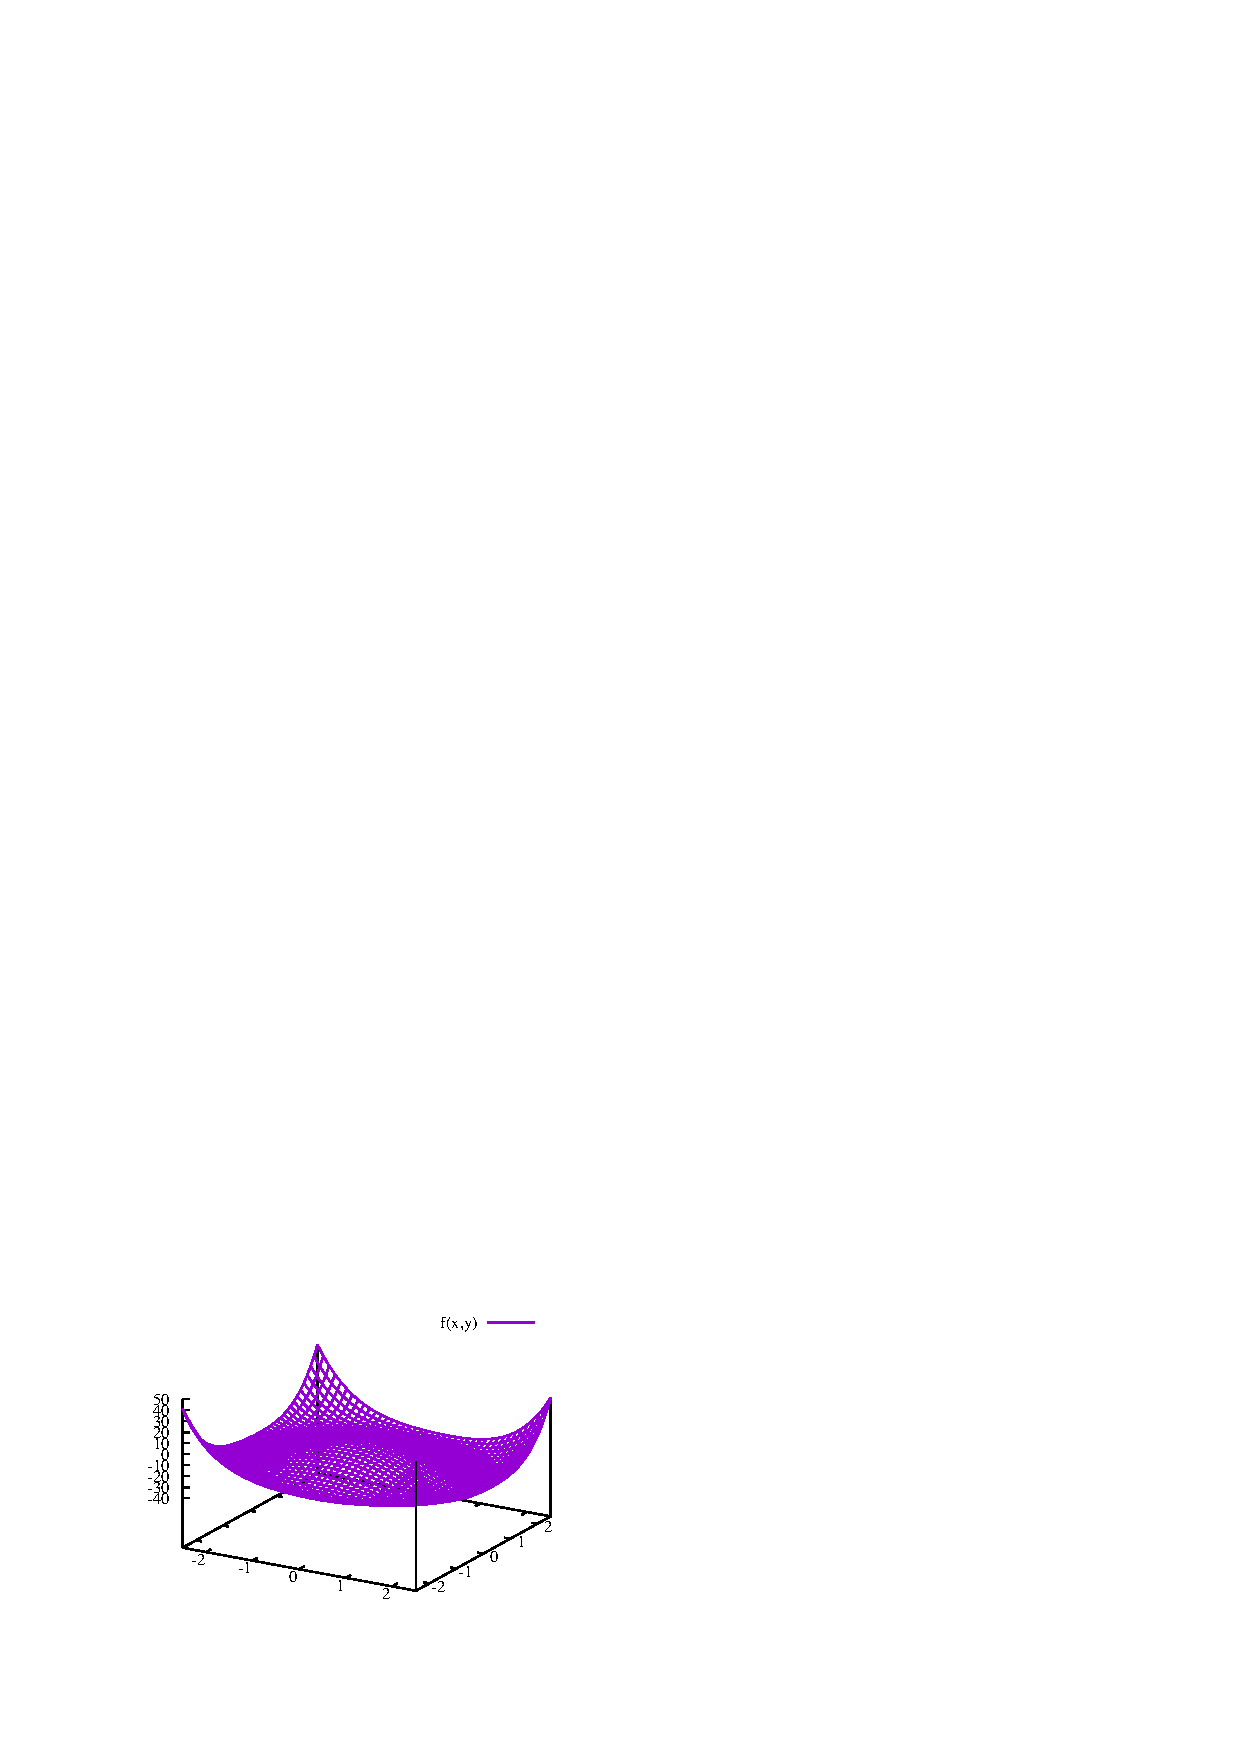
\includegraphics{image/func_2d.pdf}}
  \end{center}
\end{frame}

\begin{frame}[t,fragile]{様々な最適化手法の比較 (1/4)}
  \begin{center}
    \resizebox{.9\textwidth}{!}{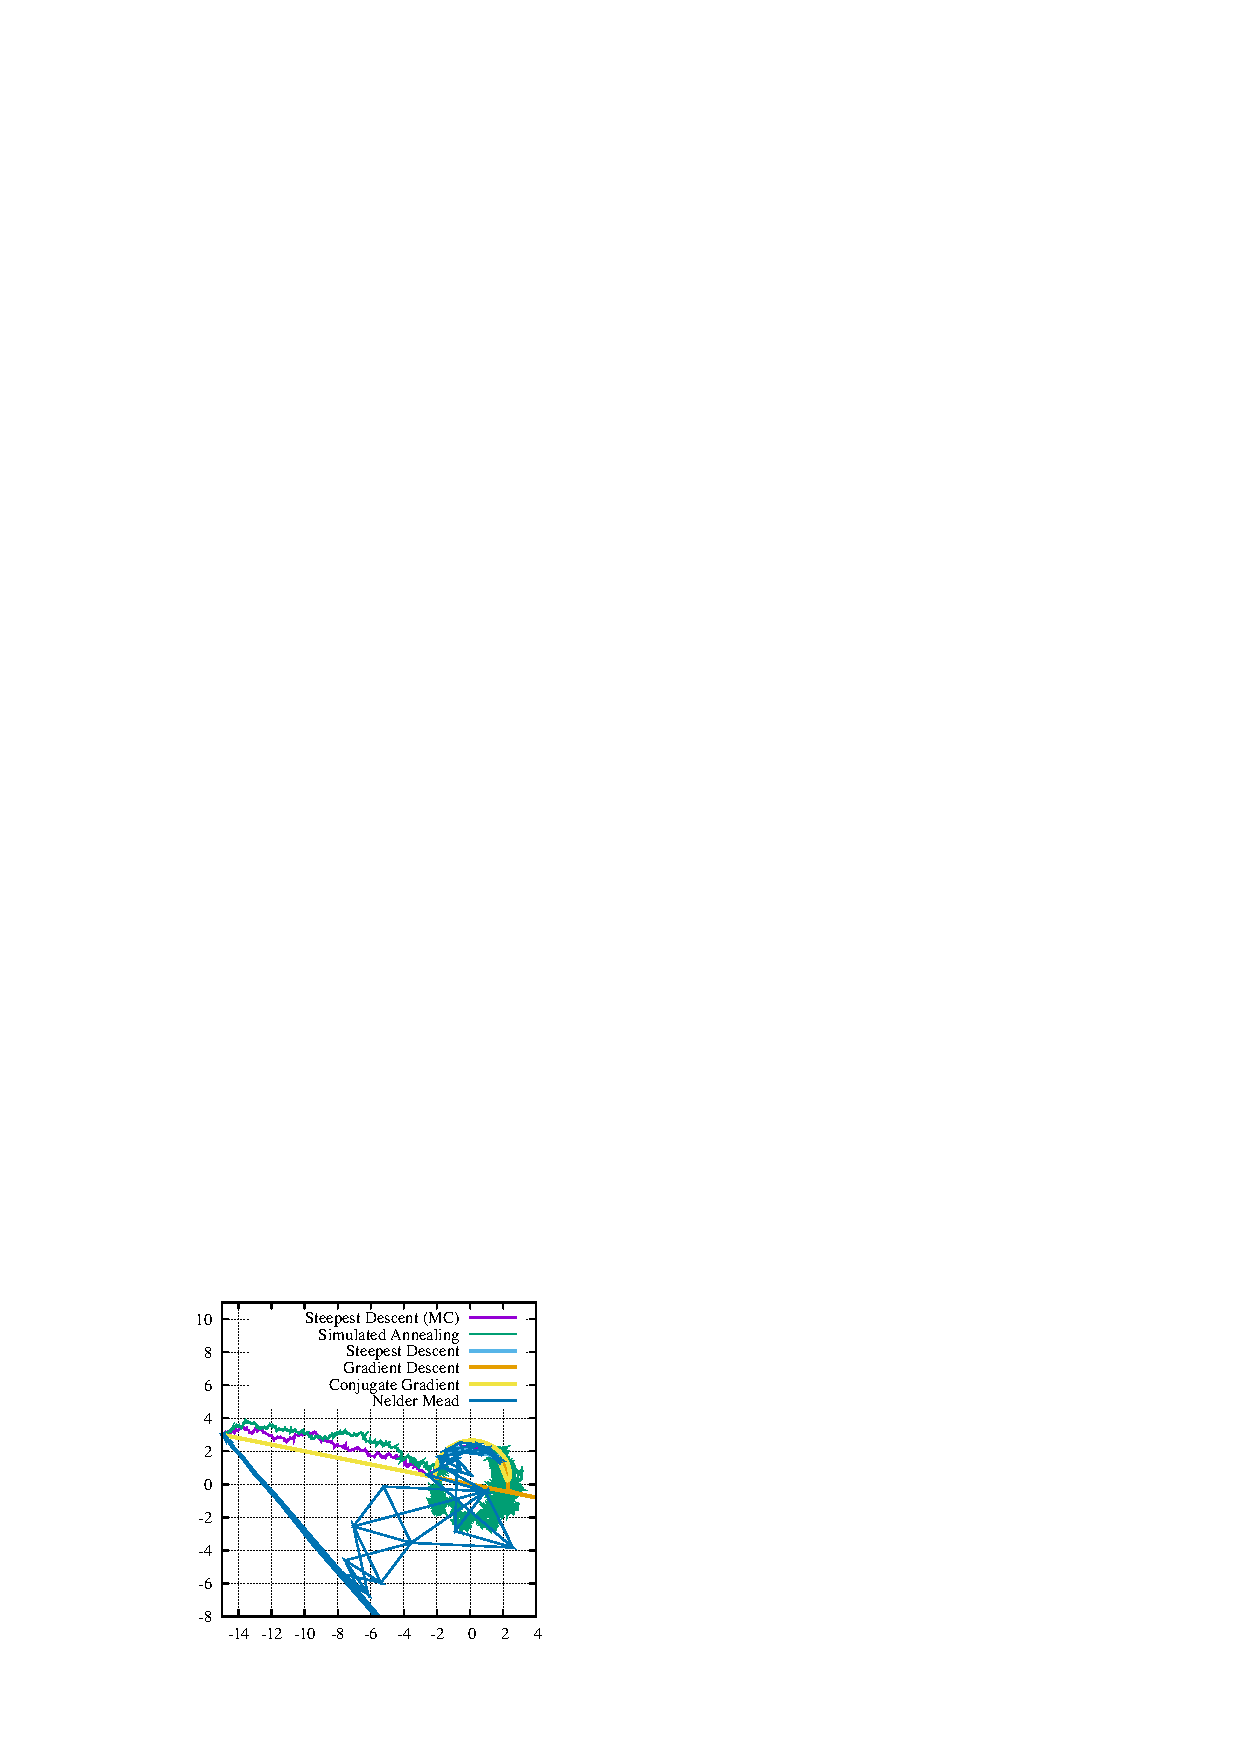
\includegraphics{image/optimization.pdf}}
  \end{center}
\end{frame}

\begin{frame}[t,fragile]{様々な最適化手法の比較 (2/4)}
  \begin{center}
    \resizebox{.9\textwidth}{!}{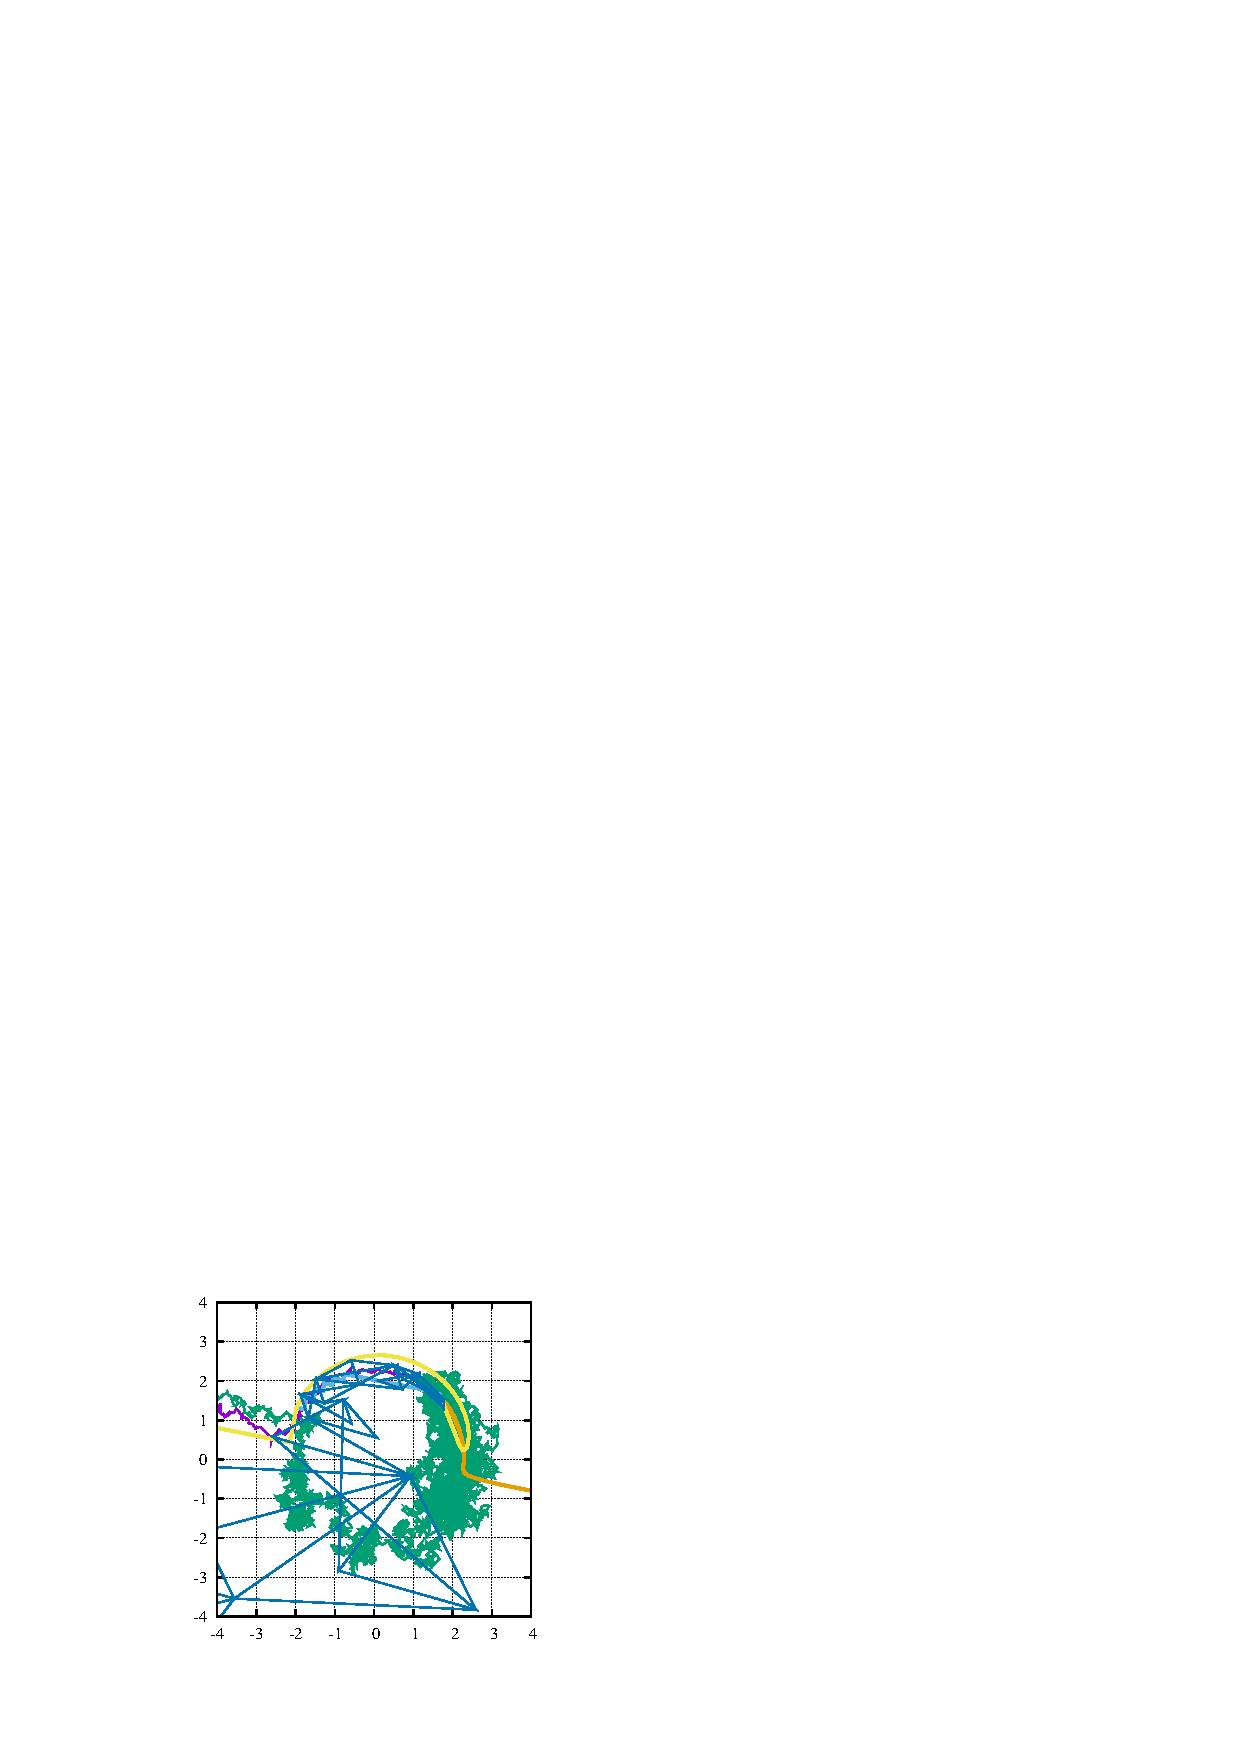
\includegraphics{image/optimization2.pdf}}
  \end{center}
\end{frame}

\begin{frame}[t,fragile]{様々な最適化手法の比較 (3/4)}
  \begin{center}
    \resizebox{.9\textwidth}{!}{\includegraphics{image/optimization3.pdf}}
  \end{center}
\end{frame}

\begin{frame}[t,fragile]{様々な最適化手法の比較 (4/4)}
  \begin{center}
    \resizebox{.9\textwidth}{!}{\includegraphics{image/optimization4.pdf}}
  \end{center}
\end{frame}

\begin{frame}[t,fragile]{真の解への近づき方}
  \begin{center}
    \resizebox{.9\textwidth}{!}{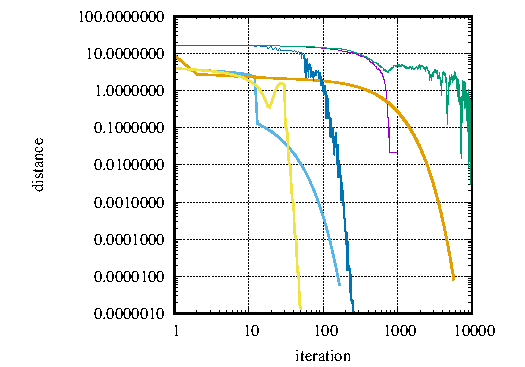
\includegraphics{image/convergence.pdf}}
  \end{center}
\end{frame}


\section{}
\begin{frame}[t]{本日の課題}
  \begin{itemize}
    %\setlength{\itemsep}{1em}
  \item 実習
    \begin{itemize}
    \item \href{https://github.com/todo-group/computer-experiments/blob/master/exercise/optimization/golden_section.c}{golden\_section.c}の内容を確認
    \item 実習課題一覧\href{https://github.com/todo-group/ComputerExperiments/releases/tag/2020a-computer2}{exercise-2.pdf}から最適化(あるいは別の)課題を選び実習
    \end{itemize}
  \item 質問はSlackの「\# 8\_最適化」あるいは他の適当と思われるチャンネルで
  \item 次回講義(12/11)の前日までにITC-LMSのアンケート「作業レポートNo.7」に回答
  \end{itemize}
\end{frame}

\end{document}
